\documentclass[12pt,a4paper]{report}

\usepackage[utf8]{inputenc}
\usepackage{geometry}
\geometry{a4paper, margin=0.7in}
\usepackage{graphicx}
\usepackage{amsmath}
\usepackage{hyperref}
\usepackage{setspace}
\usepackage{natbib}
\usepackage{array}
\usepackage{float}

\title{Actuarial Climate Index for the UK}
\author{Kgosi Ruri Molebatsi}
%\institute{Heriot-Watt University, Edinburgh}
\date{\today}

\begin{document}

\maketitle

\begin{abstract}
This report presents the development and analysis of an Actuarial Climate Index (ACI) tailored for the United Kingdom. 
Using climate data sourced from reputable meteorological agencies, we construct a composite index that captures the frequency and severity of extreme climate events relevant to actuarial risk assessment. 
The methodology involves data preprocessing, statistical analysis, and index construction, as detailed in the accompanying Jupyter notebook \texttt{final.ipynb}. 
Furthermore, the integration of the ACI into risk loading calculations is explored, demonstrating how climate-related risks can be quantitatively incorporated into insurance premium setting. 
Key findings indicate notable trends in temperature extremes, precipitation, and wind events over recent decades, with implications for insurance and risk management sectors. 
The report discusses the limitations of the current approach and suggests directions for future research to enhance the robustness and applicability of the UK ACI.
\end{abstract}

\tableofcontents
\listoffigures
\listoftables

\chapter{Introduction}

\section{Background}
Climate change has emerged as a significant challenge for societies worldwide, with increasing frequency and severity of extreme weather events posing substantial risks to economies and communities. 
The insurance and actuarial sectors are particularly affected, as climate-related events can lead to increased claims and financial instability. 
In response, there is a growing need for quantitative tools that can capture and monitor climate variability and its implications for risk assessment. 
The Actuarial Climate Index (ACI) is one such tool, designed to provide a standardized measure of climate anomalies relevant to actuarial practice.

\section{Objectives}
The primary objective of this report is to develop an Actuarial Climate Index tailored for the United Kingdom. Specific aims include:
\begin{itemize}
    \item Collecting and preprocessing relevant climate data for the UK.
    \item Constructing a composite index that reflects the frequency and severity of climate extremes.
    \item Applying statistical and machine learning techniques to analyze climate variability.
    \item Demonstrating the integration of the ACI into actuarial risk assessment and insurance pricing.
    \item Identifying limitations and proposing directions for future research.
\end{itemize}

\section{Structure of the Report}
This report is organized as follows:
\begin{itemize}
    \item \textbf{Chapter 2: Literature Review} --- Summarizes existing research on climate indices and their actuarial applications.
    \item \textbf{Chapter 3: Methodology} --- Details the data sources, preprocessing steps, and statistical methods used to construct the ACI.
    \item \textbf{Chapter 4: Results} --- Presents the findings from the analysis, including the constructed index and its interpretation.
    \item \textbf{Chapter 5: Discussion} --- Discusses the implications of the results for actuarial practice, as well as limitations of the current approach.
    \item \textbf{Chapter 6: Conclusion} --- Provides a summary of key findings, recommendations, and suggestions for future work.
    \item \textbf{Appendix} --- Contains supplementary material, data, or code relevant to the study.
\end{itemize}

\chapter{Literature Review}
\section{Relevant Studies}
Several studies have explored the development and application of climate indices for risk assessment. \citet{brooks2014actuarial} introduced the Actuarial Climate Index (ACI) for North America, providing a framework for quantifying climate-related risks relevant to the insurance industry. Their methodology combines multiple climate variables, such as temperature extremes, precipitation, and wind speed, to create a composite index.

\citet{zwiers2011climate} examined the relationship between climate variability and insurance losses, highlighting the importance of robust indices for actuarial applications. Similarly, \citet{alexander2006global} conducted a global analysis of climate extremes, offering insights into trends and variability that inform index construction.

In the UK context, \citet{kendon2014uk} analyzed changes in UK rainfall and temperature extremes, providing a foundation for region-specific climate indices. The work of \citet{palin2016future} further assessed future projections of extreme weather events in the UK, emphasizing the need for dynamic risk assessment tools.

These studies collectively inform the methodology and relevance of constructing an Actuarial Climate Index tailored for the UK.
\section{Gaps in the Literature}

\chapter{Methodology}

\section{Research Design}
This study adopts a quantitative approach to construct and analyze an Actuarial Climate Index (ACI) for the UK, integrating statistical and machine learning techniques to process climate data and assess its relevance for actuarial risk.

\section{Data Collection}
Annual climate data for the UK from 1999 to 2023 is utilized, comprising ten variables found in Table~\ref{tab:climate_factors}. Data is sourced from reputable meteorological agencies to ensure accuracy and reliability.

\begin{table}[H]
\centering
\renewcommand{\arraystretch}{1}
\setlength{\tabcolsep}{15pt}

\begin{tabular}{lll>{\raggedright\arraybackslash}p{5cm}}
\hline
\textbf{Variable Name} & \textbf{Symbol} & \textbf{Unit} & \textbf{Description} \\
\hline
Surface Wind Speed & $U$ & m/s & Annual mean wind speed at surface \\
Sea-Level Pressure & $P_{sl}$ & hPa & Annual mean sea-level atmospheric pressure \\
Relative Humidity & $RH$ & \% & Annual mean relative humidity \\
Photovoltaic Potential & $PV$ & kWh/m$^2$ & Annual mean solar energy potential \\
Maximum Temperature & $T_{max}$ & $^\circ$C & Annual mean daily maximum temperature \\
Minimum Temperature & $T_{min}$ & $^\circ$C & Annual mean daily minimum temperature \\
Precipitation Intensity & $PR$ & mm/day & Annual mean precipitation rate \\
Drought Duration & $D_{days}$ & days & Number of days with drought conditions per year \\
Frost Duration & $F_{days}$ & days & Number of days with frost conditions per year \\
Precipitation Extremes & $PR_{ext}$ & days & Number of days with extreme precipitation per year \\
\hline
\end{tabular}
\caption{Climate Variables Used in the UK ACI Construction}
\label{tab:climate_factors}
\end{table}

\section{Data Preprocessing}
Each climate variable is transformed into a \textbf{standardized anomaly} to ensure comparability across different units and scales. This involves subtracting the long-term mean and dividing by the standard deviation for each variable over the study period. The resulting standardized anomalies have zero mean and unit variance, facilitating unbiased multivariate analysis.

\section{Data Analysis}

\subsection{Principal Component Analysis (PCA)}
Principal Component Analysis (PCA) is applied to the matrix of standardized anomalies to reduce dimensionality and identify dominant modes of interannual climate variability. PCA projects the original correlated variables onto new orthogonal axes (principal components) that sequentially maximize explained variance.

Mathematically, PCA decomposes the covariance matrix \( \mathbf{C} \) of the standardized anomaly data as:
\[
\mathbf{C} = \mathbf{V} \mathbf{\Lambda} \mathbf{V}^\top,
\]
where \( \mathbf{V} \) is the matrix of eigenvectors (loadings), and \( \mathbf{\Lambda} \) is the diagonal matrix of eigenvalues representing the variance explained by each principal component.

The first \(k\) principal components (PCs) are selected such that they collectively explain approximately 80\% of the total variability in the standardized climate anomaly data. This approach preserves the majority of the multivariate climate information while reducing dimensionality, enabling efficient and robust forecasting. Formally, the Anomaly Climate Index at time \(t\) can be reconstructed as
\[
\hat{\mathbf{Z}}_t = \sum_{i=1}^k \mathbf{v}_i \, PC_i(t),
\]
where \(\mathbf{v}_i\) is the loading vector for the \(i\)-th principal component and \(PC_i(t)\) is the score of the \(i\)-th component at time \(t\).

\begin{figure}[H]
    \centering
    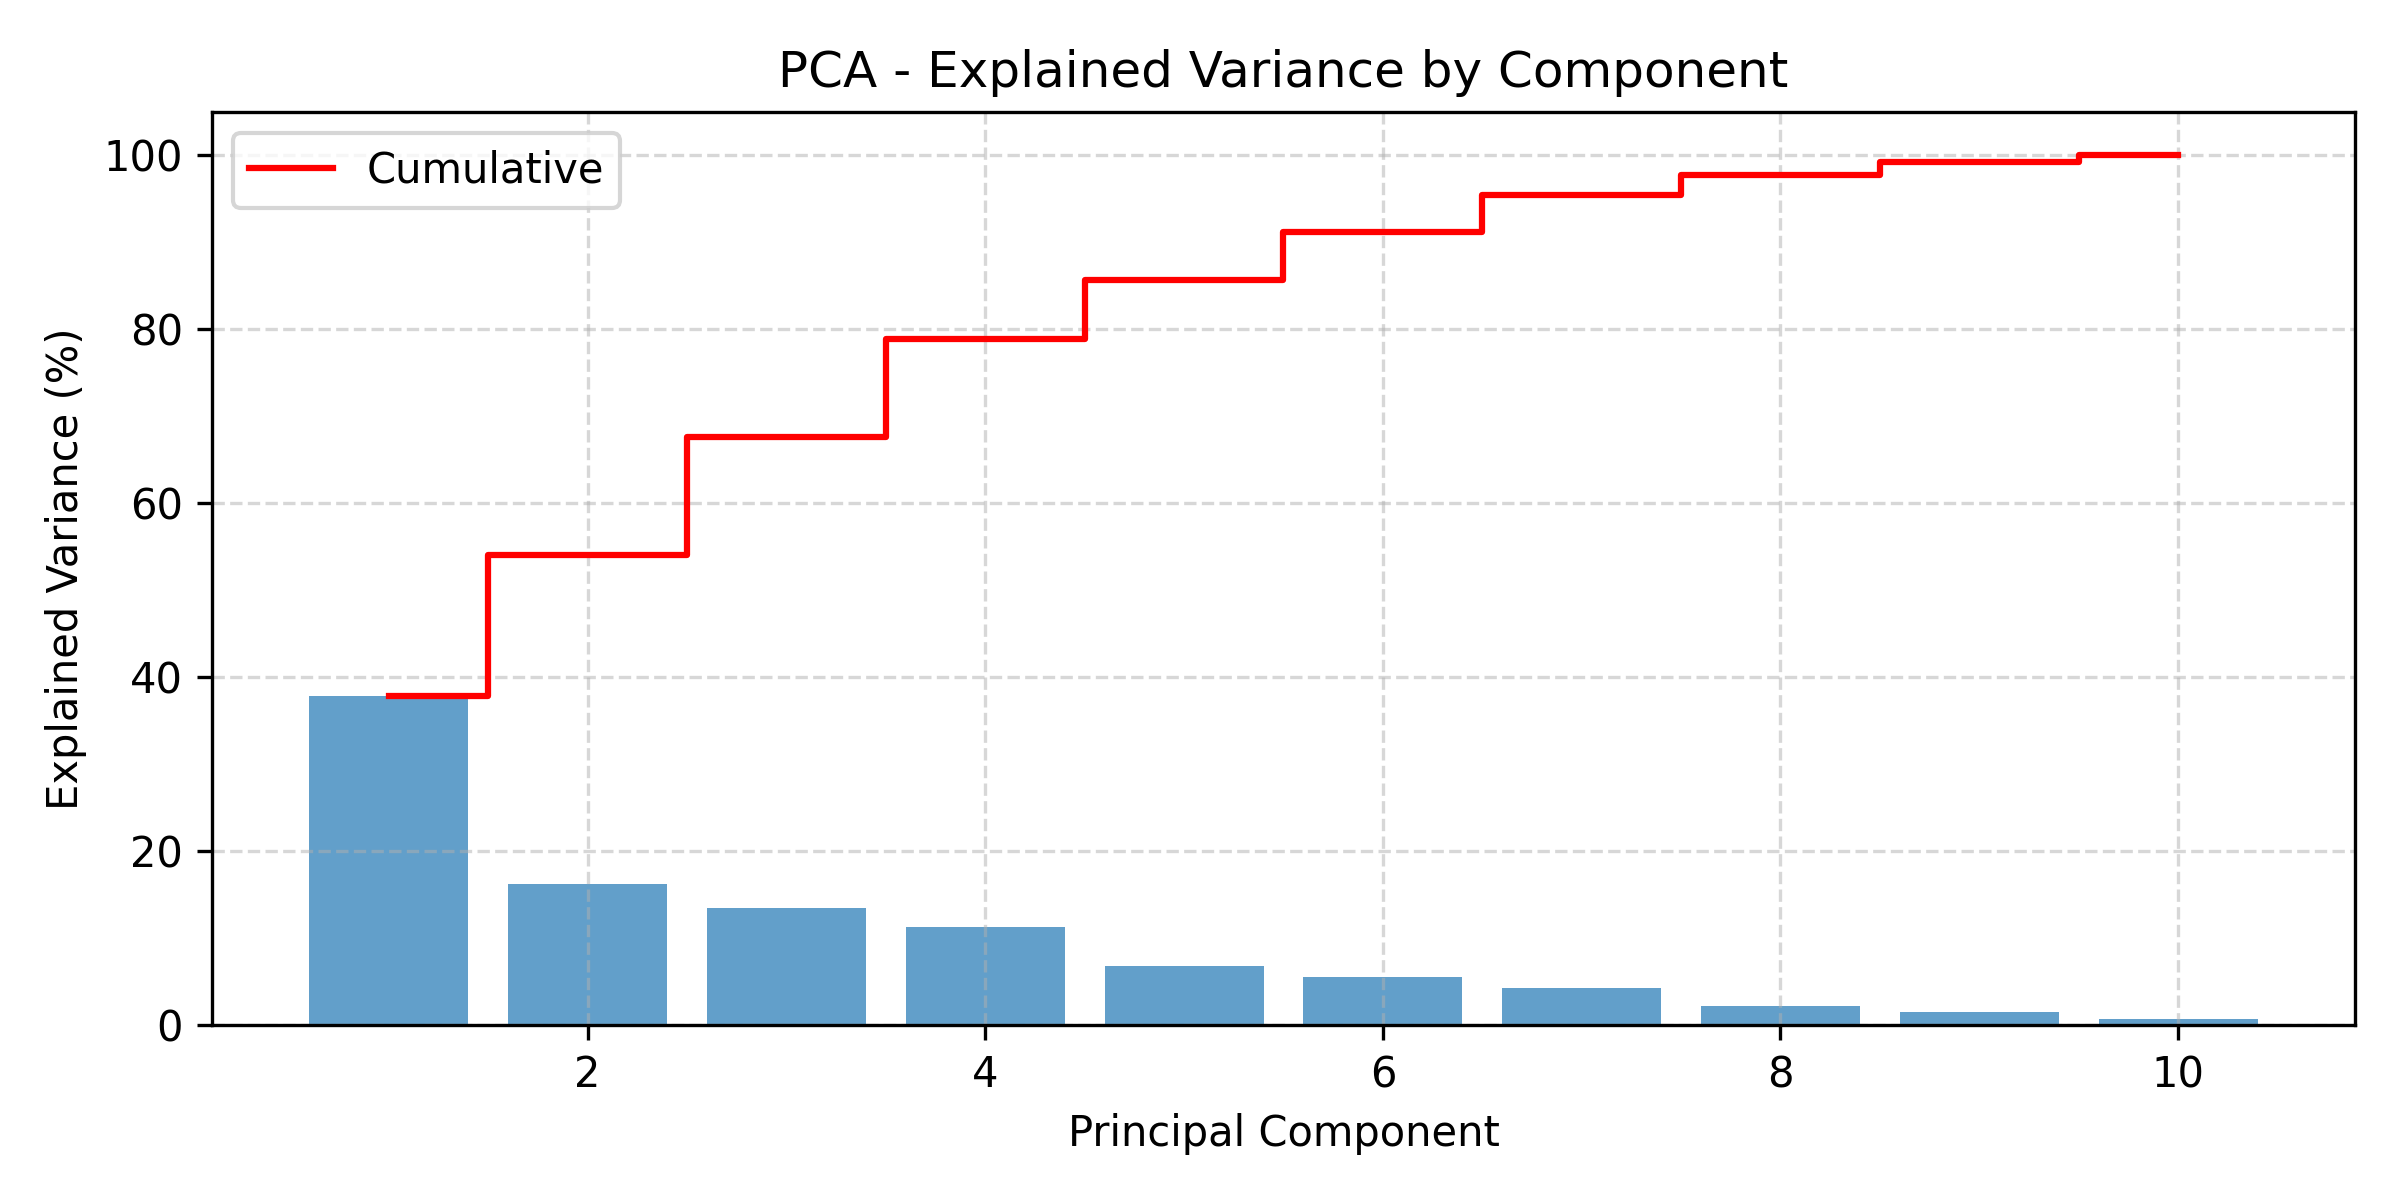
\includegraphics[width=0.7\textwidth]{pca_explained_variance_report.png}
    \caption{Explained variance ratio of each principal component from PCA applied to standardized UK climate anomalies (1999--2023). The first few components capture the majority of the variance, justifying dimensionality reduction for index construction.}
    \label{fig:pca_explained_variance}
\end{figure}
\subsection{Interpretation and Validation}
The loadings of the selected PCs provide insight into which climate variables most strongly influence the index, offering interpretability crucial for actuarial applications. Sensitivity analyses are conducted by performing PCA on sub-periods to evaluate the stability of loadings and explained variance. 
Additionally, bootstrapping methods generate confidence intervals for the loadings and principal components, quantifying uncertainty inherent in the index construction.

\subsection{Forecasting with Quantum Kernel Long Short-Term Memory (QK-LSTM) Networks}
To forecast future values of the ACI represented by multiple principal components, a hybrid Quantum Kernel and Long Short-Term Memory (QK-LSTM) neural network is employed. 
This advanced architecture integrates quantum kernel methods with classical LSTM networks to enhance the modeling of complex temporal dependencies and nonlinear relationships in climate data \citep{schuld2019quantum, li2022quantum}.

Quantum kernels project classical input data into high-dimensional Hilbert spaces using parameterized quantum circuits, capturing intricate nonlinearities that classical kernels may not detect. The quantum kernel between two inputs \(x\) and \(x'\) is given by
\[
K(x, x') = |\langle \psi(x) | \psi(x') \rangle|^2,
\]
where \(\psi(\cdot)\) denotes the quantum feature embedding.

The time series of the selected PCs is embedded into this quantum space to produce kernel matrices representing nonlinear similarities among temporal observations. These kernel-derived features are then input into an LSTM network, which captures the temporal dynamics and sequential dependencies of the climate anomaly data.

The QK-LSTM model leverages the combined strengths of quantum-enhanced feature representations and the powerful sequence modeling capabilities of LSTM networks to improve forecast accuracy. The predicted future PC values are then used to reconstruct the climate anomaly patterns through the PCA loadings, allowing a comprehensive forecast of the ACI.

\textbf{Strength of LSTM:}  
LSTM neural networks are designed to model complex, nonlinear temporal dependencies by maintaining gated memory cells that control information flow over long sequences. This makes them particularly well-suited for capturing the dynamic and potentially non-stationary behavior of climate indices such as the ACI.

\begin{table}[H]
\centering
\renewcommand{\arraystretch}{1}
\setlength{\tabcolsep}{15pt}
\begin{tabular}{ll}
\hline
\textbf{Step} & \textbf{Description} \\
\hline
1. Data Preparation & Standardize and structure PC time series into input/output sequences \\
2. Quantum Kernel Embedding & Apply quantum feature mapping and compute kernel matrices \\
3. Model Initialization & Define LSTM architecture (layers, units, activation functions) \\
4. Training & Fit the QK-LSTM model to historical PC data using backpropagation \\
5. Validation & Evaluate model performance on a hold-out validation set \\
6. Forecasting & Generate future PC predictions using the trained QK-LSTM \\
7. Reconstruction & Combine predicted PCs with loadings to reconstruct climate anomalies \\
8. Uncertainty Estimation & (Optional) Use dropout or ensemble methods for predictive intervals \\
\hline
\end{tabular}
\caption{Algorithm for QK-LSTM-based ACI Forecasting}
\label{tab:lstm_algorithm}
\end{table}

This hybrid QK-LSTM framework provides a promising, data-driven approach to forecasting the ACI, capturing nonlinearities and temporal patterns beyond traditional linear models and purely classical neural networks. It advances the predictive capabilities required for actuarial climate risk assessment and planning.

\section{Technical Methods}
This section details the statistical and computational techniques used, including data standardization, PCA, sensitivity analysis, bootstrapping, and Bayesian time series modeling.

\section{Integration with Actuarial Risk Assessment}
The ACI is intended as a compact, multivariate indicator of climate anomalies relevant for insurance and risk management. Future work will focus on integrating the index with loss data models to evaluate its predictive power in actuarial contexts, including claims frequency and severity associated with extreme climate events.

\chapter{Results}
\section{Findings}
\section{Interpretation}

\chapter{Discussion}
\section{Implications}
\section{Limitations}

\chapter{Conclusion}
\section{Summary}
\section{Recommendations}
\section{Future Work}

\bibliographystyle{plainnat}
\bibliography{references}

\appendix
\chapter{Appendix}
Additional material, data, or code.

\end{document}